\documentclass[a4paper]{article}     
\usepackage{amsfonts}
\usepackage{amsmath}
\usepackage{amssymb}
\usepackage{graphicx}

\begin{document}

\noindent \large Auteur: Ayoub Jaaouan \\
\noindent \large Studierichting: Informatica\\
\noindent \large Oefeningenreeks 3G nr. 7.5\\

\medskip

\normalsize

$f(x) = (x-1)(x-2)(x-3)$ \\

Nulpunten: \\

$f(x) = 0 \Rightarrow f(1) = (1-1)(1-2)(1-3) = 0 \Rightarrow x = 1$ \\

$f(x) = 0 \Rightarrow f(2) = (2-1)(2-2)(2-3) = 0 \Rightarrow x = 2$ \\

$f(x) = 0 \Rightarrow f(3) = (3-1)(3-2)(3-3) = 0 \Rightarrow x = 3$ \\

\bigskip

$f'(x) = (3x^2-12x+11) $\\

Extrema: \\

$D = 12$\\

$x_1 = \dfrac{12+\sqrt{12}}{6}$\\

$x_2 = \dfrac{12-\sqrt{12}}{6}$\\



\bigskip

$f''(x) = (6x-12) $\\

Buigpunten: \\

$f''(x) = 0 \Rightarrow f''(2) =  (6\cdot2-12) = 0 \Rightarrow x = 2 $ \\

Tekenonderzoek.: \\

\begin{tabular}{c|ccccccccccc}
$x$				&		& $1$ &  & $\dfrac{12-\sqrt{12}}{6}$ &  & $2$ &  & $\dfrac{12+\sqrt{12}}{6}$ &  & $3$ & \\ \hline
$f(x)$		& $-$ & $0$ & $+$ & $+$ & $+$ & $0$ & $-$ & $-$ & $-$ & $0$ & $+$ \\
$f'(x)$		& $+$ & $+$ & $+$ & $0$ & $-$ & $-$ & $-$ & $0$ & $+$ & $+$ & $+$ \\
$f''(x)$	& $-$ & $-$ & $-$ & $-$ & $-$ & $0$ & $+$ & $+$ & $+$ & $+$ & $+$ \\ \hline
$f(x)$		& $\nearrow$ & $\nearrow$ & $\nearrow$ & $M\left(\dfrac{2\sqrt{3}}{9}\right)$ & $\searrow$ & $\searrow$ &$\searrow$ & $m\left(\dfrac{-2\sqrt{3}}{9}\right)$ & $\nearrow$ & $\nearrow$ & $\nearrow$ \\
					& $\frown$ & $\frown$ & $\frown$ & $\frown$ & $\frown$ & $0$ & $\smile$ & $\smile$ & $\smile$ & $\smile$ & $\smile$ \\
\end{tabular}  \\

\medskip



\begin{figure}[h]
    \centering
    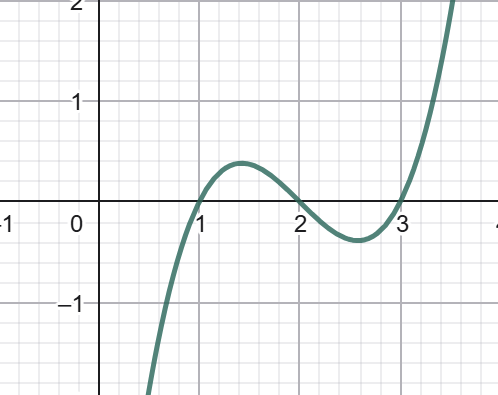
\includegraphics[width=0.5\textwidth]{3G-7.5-ayoub.jaaouan.INF.png}
\end{figure}

\begin{thebibliography}{999}
%\bibitem{a} Referentie
\end{thebibliography}
\end{document} 
